\documentclass[12pt,a4paper,twoside]{book}
\usepackage{graphicx}
\usepackage{setspace} % espaciado doble para texto, simple para pies de página, subtítulos, etc.
\usepackage{natbib} % sustituto de 'hypernat' que funciona en Windows.
\usepackage[catalan]{babel}
\usepackage[utf8]{inputenc}
\usepackage{color}
\usepackage{hhline} % estilos extendidos para tablas
\usepackage{multirow}
\usepackage{subfigure}
\usepackage{acronym}
\usepackage{hyperref}
\usepackage{amsmath,amssymb}
\usepackage{fancyhdr}
\usepackage{epsfig, amsmath}
\usepackage{algorithm}
\usepackage{algorithmic}
\usepackage{url}


% configuraciones generales
\hypersetup{
linktocpage=true,
colorlinks=true,
linkcolor=blue,
citecolor=blue,
}
\definecolor{Hgray}{gray}{0.6}

\newenvironment{definition}[1][Definición]{\begin{trivlist}
\item[\hskip \labelsep {\bfseries #1}]}{\end{trivlist}}

\setlength{\topmargin}{0cm}
\setlength{\textheight}{23cm}
\setlength{\textwidth}{17cm}
\setlength{\oddsidemargin}{0cm}
\setlength{\evensidemargin}{0cm}
\setlength{\headheight}{1cm}

% indica que las 'sub-sub-secciones' están numeradas y aparecen en el índice
\setcounter{secnumdepth}{3}
\setcounter{tocdepth}{2}

% configuraciones para código
\renewcommand{\algorithmicrequire}{\textbf{Entrada:}}
\renewcommand{\algorithmicensure}{\textbf{Salida:}}

%%%%%%%%%%%%
% DOCUMENTO %
%%%%%%%%%%%%
\begin{document}

\renewcommand{\thesection}{\thechapter} % Sección numerada como Capítulo.Subseccion


% portada
\input{0_titulo.tex}
\newpage
% resumen
\input{0_resumen.tex}
\newpage

\pagestyle{fancy}
\renewcommand{\chaptermark}[1]{ \markboth{#1}{}}
\renewcommand{\sectionmark}[1]{\markright{ \thesection.\ #1}}
\lhead[\fancyplain{}{\bfseries\thepage}]{\fancyplain{}{\bfseries\rightmark}}
\rhead[\fancyplain{}{\bfseries\leftmark}]{\fancyplain{}{\bfseries\thepage}}
\cfoot{}

% tabla de contenidos
\cleardoublepage
\phantomsection
\addcontentsline{toc}{chapter}{Índex}
\tableofcontents
% lista de figuras
\cleardoublepage
\phantomsection
\addcontentsline{toc}{chapter}{Llista de figures}
\listoffigures


\thispagestyle{empty}

\pagenumbering{arabic}

\pagestyle{fancy}
\renewcommand{\chaptermark}[1]{ \markboth{#1}{}}
\renewcommand{\sectionmark}[1]{\markright{ \thesection.\ #1}}
\lhead[\fancyplain{}{\bfseries\thepage}]{\fancyplain{}{\bfseries\rightmark}}
\rhead[\fancyplain{}{\bfseries\leftmark}]{\fancyplain{}{\bfseries\thepage}}
\cfoot{}

\onehalfspacing

\chapter{Introducció}

\subsection{Context i motivació}
\sloppy

En els darrers anys, els algorismes han revolucionat el món de la inversió, transformant el mercat bursàtil. No obstant això, la majoria d'aquests models es basen principalment en dades històriques, com preus, volums i altres indicadors quantitatius. Tot i la seva utilitat, aquest enfocament ignora factors externs que poden influir de manera significativa en els mercats, com ara decisions polítiques o la percepció pública davant d'esdeveniments globals. Així, es deixa de banda una font d'informació clau: l'actualitat financera, política, empresarial i econòmica que influeix en el mercat des de l'exterior.

L'objectiu d'aquest projecte és explorar com la integració d'informació extreta de notícies pot millorar la capacitat predictiva i la presa de decisions d'un agent d'inversió basat en Aprenentatge per Reforç Profund (Deep Reinforcement Learning, en endavant DRL). Es pretén analitzar si la combinació de dades quantitatives (com preus, volums i altres indicadors històrics) i qualitatives pot oferir un avantatge respecte als enfocaments tradicionals basats exclusivament en dades estructurades.

Les dades qualitatives utilitzades en aquest projecte provenen de notícies, que es processen mitjançant tècniques avançades de tractament del llenguatge natural (Natural Language Processing, en endavant NLP). Aquestes tècniques inclouen la representació semàntica de paraules amb Word2Vec, la modelització de temes i l'anàlisi de sentiments.

La rellevància d'aquest estudi rau en el fet que vivim en un món interconnectat, on la informació es transmet de manera gairebé instantània. Canvis polítics, conflictes geopolítics o notícies rellevants sobre grans corporacions poden desencadenar reaccions immediates als mercats. Aquest escenari dinàmic exigeix que les estratègies d'inversió siguin més flexibles, adaptatives i capaces d'incorporar informació contextual actualitzada.

El projecte proposa el desenvolupament d'un agent d'inversió basat en DRL que integri tant dades financeres com notícies processades mitjançant tècniques de NLP. S'avaluaran tres algoritmes de DRL (DQN, PPO i SAC) per determinar quin s'adapta millor a aquest enfocament. La comparació es durà a terme mitjançant mètriques financeres com el Sharpe Ratio, el Drawdown i el retorn esperat, amb l'objectiu de demostrar si l'ús d'informació qualitativa pot millorar la presa de decisions d'inversió i com varien els resultats entre cadascun dels models.

A nivell personal, aquest treball representa una oportunitat per aprofundir i formar-me en dos àmbits que em resulten molt interessants: les finances i l'aprenentatge per reforç. Tot i que no disposo d'una formació financera extensa, sempre m'ha interessat comprendre quins factors impulsen les fluctuacions dels mercats.

D'altra banda, l'aprenentatge per reforç és una branca del machine learning que, tot i allunyar-se del que faig habitualment, considero rellevant per a la presa de decisions autònomes en entorns de risc, com els mercats financers, on tradicionalment els humans han pres decisions basant-se més en la seva experiència i coneixement que únicament en les dades disponibles. M'agrada el repte d'haver de tractar les dades qualitatives mitjançant tècniques de NLP per integrar aquesta informació al model per proporcionar a l'agent d'inversió un context més ampli i precís.

\subsection{Objectius}
L'objectiu principal d'aquest treball és desenvolupar un agent d'inversió basat en Aprenentatge per Reforç Profund (DRL) que integri informació financera i notícies processades mitjançant tècniques avançades de NLP per a la presa de decisions d'inversió. L'agent serà entrenat en un entorn de simulació de mercat i s'avaluarà el seu rendiment comparant-lo amb estratègies tradicionals. Aquest objectiu principal comporta els següents objectius parcials

\begin{itemize}
    \item \textbf{Processament i transformació de les dades relacionades amb notícies financeres}
    \begin{itemize}
        \item[--] Obtenció de les notícies a través de les APIs proporcionades per diferents diaris.
        \item[--] Implementació de tècniques de NLP per processar els titulars de les notícies.
        \item[--] Integració de les dades processades en l'entorn de simulació per utilitzar-les en la presa de decisions de l'agent.
    \end{itemize}

    \item \textbf{Disseny de l'entorn de simulació}
    \begin{itemize}
        \item[--] Creació de l'entorn de mercat financer utilitzant OpenAI Gym\cite{OpenAIGym}.
        \item[--] Definició de l'espai d'estats, incloent-hi indicadors financers i les dades relacionades amb les notícies.
        \item[--] Definició de les accions i disseny de la funció de recompensa.
    \end{itemize}

    \item \textbf{Implementació i comparació de diferents algoritmes de DRL}
    \begin{itemize}
        \item[--] Creació i entrenament de tres models d'Aprenentatge per Reforç: DQN, PPO i SAC.
        \item[--] Ajust d'hiperparàmetres per optimitzar el procés d'aprenentatge.
        \item[--] Comparació dels tres models.
    \end{itemize}

    \item \textbf{Avaluació del rendiment de l'agent i comparació amb estratègies tradicionals}
    \begin{itemize}
        \item[--] Mesura del rendiment de l'agent amb les mètriques Sharpe Ratio, Drawdown i retorn esperat.
        \item[--] Comparació del model DRL amb models basats únicament en indicadors tècnics (sense noticies).
        \item[--] Anàlisi de l'impacte de la integració de notícies en les decisions de l'agent, avaluant si aporta un avantatge competitiu.
    \end{itemize}
\end{itemize}

\subsection{Sostenibilitat, diversitat i reptes ètics/socials}

Aquest projecte es centra en la implementació d'un model algorítmic per a la inversió financera. Tot i que no es preveu un efecte directe en aspectes com la sostenibilitat, l'ètica o la diversitat, aquests factors poden estar presents de manera indirecta.

\begin{description}
    \item[Sostenibilitat] L'entrenament de models d'aprenentatge profund requereix una quantitat significativa de recursos computacionals, això va directament relacionat amb un consum energètic. Aquest impacte es pot minimitzar optimitzant els entrenaments i reduint el nombre de simulacions innecessàries.
    \item[Comportament ètic la responsabilitat social] Les dades utilitzades en el projecte són públiques, per la qual cosa no planteja problemes de privacitat o seguretat. No obstant això, aquests poden ser difícils d'interpretar, ja que sovint funcionen com una 'caixa negra' en la presa de decisions. Per tal de mitigar aquest fet, es posarà èmfasi en l'anàlisi dels resultats i en la comprensió del comportament de l'agent.
    \item[Diversitat, gènere i drets humans] Aquest treball no té un impacte directe en aquests àmbits ja que se centra en la presa de decisions financeres basada en dades. No obstant això, cal tenir en compte que els models NLP poden heretar biaixos de les fonts d'informació utilitzades. Per evitar-ho, s'utilitzaran notícies de mitjans diversos per minimitzar qualsevol tendència ideològica que pugui afectar les decisions de l'agent.
\end{description}

\subsection{Enfocament i metodologia}

Aquest projecte segueix una estratègia de recerca experimental, centrada en el desenvolupament i avaluació d'un agent d'inversió basat en DRL. La metodologia es basa en la integració de dades estructurades, com preus i volums obtinguts mitjançant Yahoo Finance\cite{YahooFinance}, i dades no estructurades, com notícies extretes de The Guardian\cite{TheGuardian} i The New York Times\cite{NYTimes}. Aquestes notícies es processaran utilitzant tècniques avançades de processament de llenguatge natural, com Word2Vec per identificar el contingut semàntic, topic modeling (LDA) per descobrir temes subjacents, i anàlisi de sentiments per capturar el to dels titulars.

L'entorn de simulació es desenvoluparà amb OpenAI Gym, integrant tant les dades financeres com les característiques extretes de les notícies. Es definirà un sistema de recompenses amb l'objectiu de guiar l'agent cap a les millors decisions d'inversió. Per a la implementació dels models de DRL, s'utilitzaran tres algoritmes principals: DQN (Deep Q-Network), PPO (Proximal Policy Optimization) i SAC (Soft Actor-Critic). Durant aquesta fase, es realitzarà un ajust d'hiperparàmetres per optimitzar el rendiment dels models.

L'avaluació dels models es durà a terme mitjançant mètriques financeres com el Sharpe Ratio, el Drawdown i el retorn esperat. A més, es compararan els resultats amb estratègies tradicionals, per avaluar fins a quin punt la incorporació de notícies aporta un avantatge competitiu a l'agent. Tota la implementació es realitzarà en Python\cite{Python}, aprofitant llibreries especialitzades.

\subsection{Planificació}
La planificació d'aquest treball s'ha fet d'acord a la planificació proposada al pla docent.
\begin{itemize}

    \item  \textbf{Investigació}: Aquesta primera etapa del projecte se centra en adquirir coneixements sobre el mercat borsari i en la recerca de fonts de dades accessibles que puguin aportar un valor significatiu al treball.

    \item \textbf{Definició i introducció}: En aquesta fase, es defineix la planificació i els objectius del projecte, així com la justificació i rellevància d'aquests objectius dins del context de l'aprenentatge per reforç aplicat als mercats financers.

    \item \textbf{Revisió de l'estat de l'art}: Cerca i anàlisi de la literatura i treballs previs relacionats amb l'aprenentatge per reforç aplicat a l'àmbit d'aquest treball.
    \item \textbf{Extracció de dades i creació del l'entorn}: Desenvolupament del codi necessari per a l'extracció i processament de les dades que s'utilitzaran durant el projecte. Això inclou l'obtenció de dades d'APIs i altres fonts, així com el seu tractament i modelatge per a integrar-les en l'entorn de simulació. Paral·lelament, es desenvoluparà l'entorn de simulació basat en OpenAI Gym, definint l'espai d'observació, les accions disponibles i la funció de recompensa del model.

    \item \textbf{Implementació i validació}: Implementació dels algoritmes de DRL que s'utilitzaran i la seva posterior validació. Es configuraran els models seleccionats, i s'entrenaran dins l'entorn de simulació. La validació es durà a terme mitjançant diferents mètriques d'avaluació.

    \item \textbf{Redacció de la memòria}: Elaboració del document final del treball i redacció de les conclusions.

\end{itemize}

\begin{figure}[H]
	\centering
	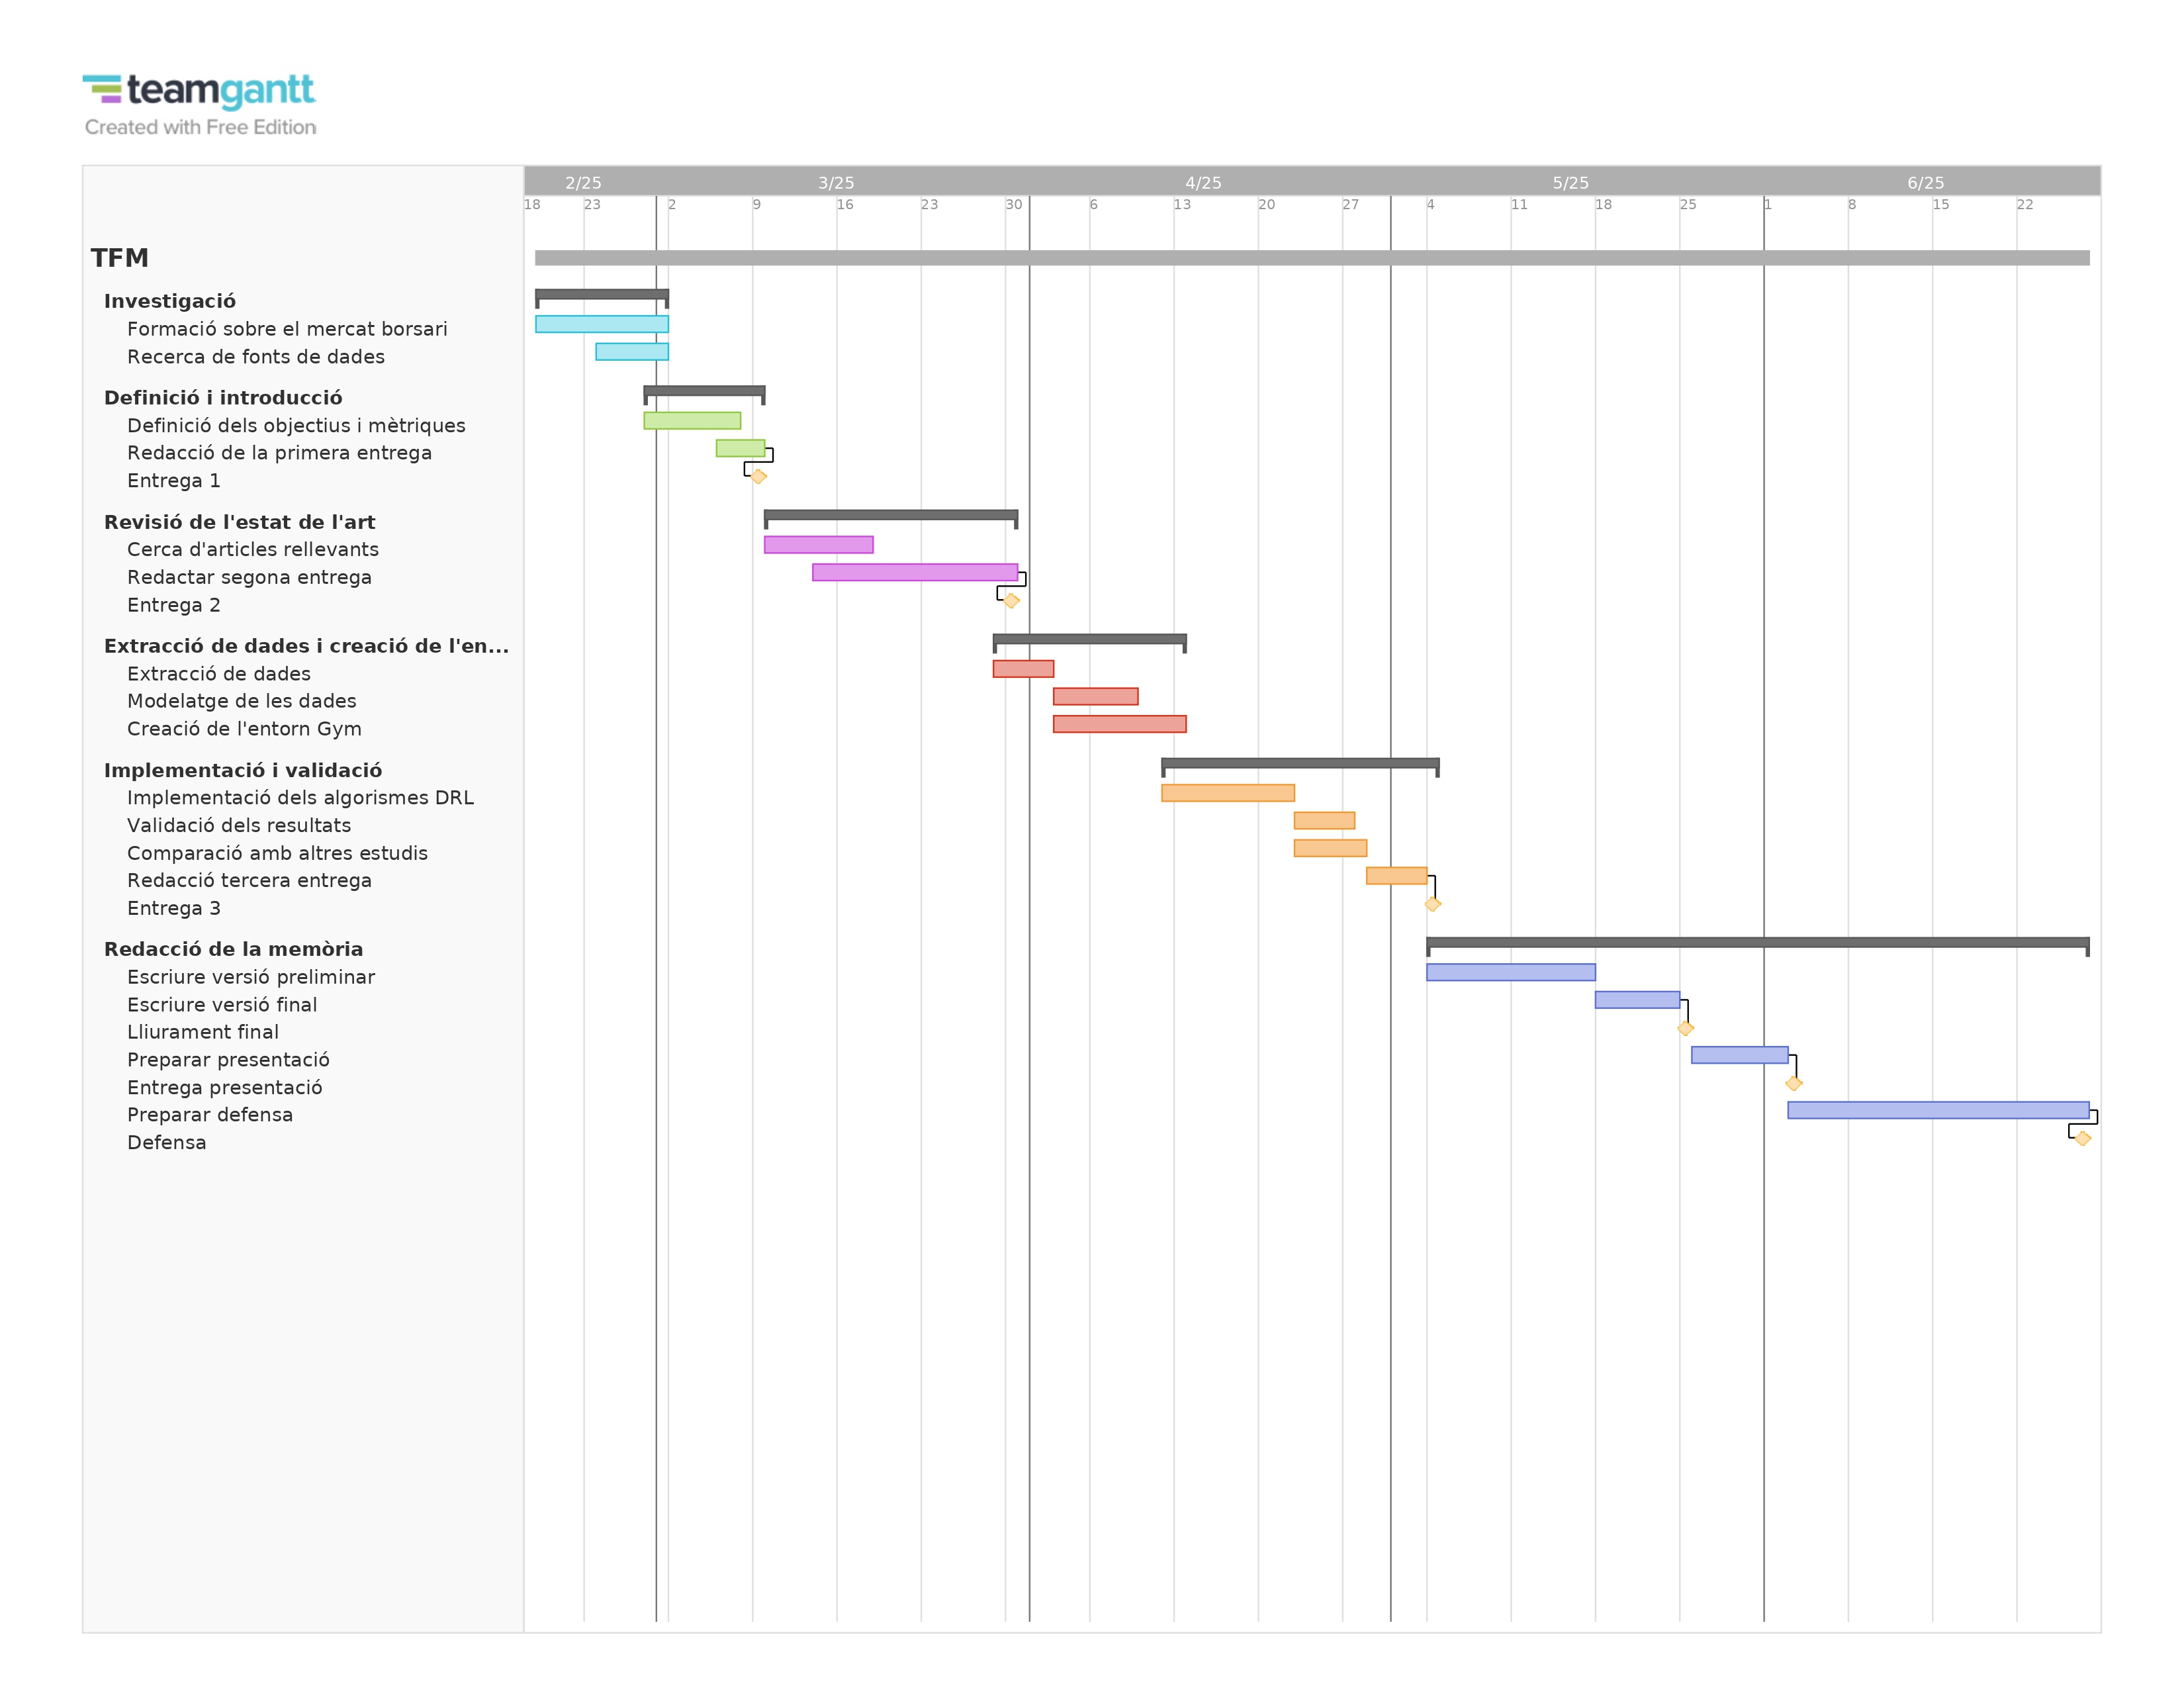
\includegraphics[width=1\textwidth]{figs/planning.jpg}
	\caption{Planificació del treball creada amb l'eina TeamGantt\cite{TeamGantt}.}
	\label{fig:context-anoni1}
\end{figure}


\subsection{Resum dels productes del projecte}

Els resultats d'aquest projecte inclouran el desenvolupament d'un agent d'inversió basat en Aprenentatge per Reforç Profund capaç d'integrar dades financeres i notícies processades mitjançant tècniques de NLP com , topic modeling (LDA) i anàlisi de sentiments. L'agent s'entrenarà en un entorn de simulació desenvolupat amb OpenAI Gym, on podrà analitzar dades de mercat i informació qualitativa per optimitzar la seva presa de decisions.

A més, es crearà una pipeline de processament de notícies per obtenir, netejar i transformar titulars de mitjans com The Guardian i The New York Times en una representació numèrica adequada per al model. Finalment, es durà a terme una avaluació detallada dels algorismes DQN, PPO i SAC mitjançant mètriques financeres com el Sharpe Ratio, Drawdown i retorn esperat, amb l'objectiu d'analitzar l'impacte de la integració de notícies en la presa de decisions.

% \subsection{Breu descripció de la resta de capítols de l'informe.}
% TBD

\chapter{Estat de l'art}

En aquest capítol s'exposen els fonaments teòrics i els treballs previs relacionats amb el desenvolupament d'agents d'inversió basats en Aprenentatge per Reforç Profund aplicats als mercats financers. Primerament, es revisa el concepte de trading i l'evolució cap al trading algorísmic per comprendre d'on sorgeix la necessitat d'aquestes noves estrategies. A continuació, es presenten els principis bàsics del DRL, juntament amb els algoritmes específics (Deep Q-Network, Proximal Policy Optimization i Soft Actor-Critic) que s'utilitzaran en aquest projecte.

A més, s'aborda la integració de dades qualitatives, com són en aquest cas les notícies, en els sistemes de decisió. També s'hi descriuen les principals tècniques de Processament del Llenguatge Natural que s'aplicaran en aquest treball. Finalment, es fa un repàs dels estudis i iniciatives que combinen DRL i NLP en l'àmbit financer.

\subsection{Introducció al trading}
\sloppy

Els mercats financers són un dels motors principals de l'economia global, ja que permeten la compra i venda d'actius com ara accions, bons, productes derivats o divises \cite{InvestopediaFinance}. Aquesta activitat permet a empreses i governs obtenir finançament, mentre que els inversors poden buscar rendiments ajustats al risc. Històricament, la presa de decisions en aquests mercats es basava en l'anàlisi fonamental, que se centra en l'estudi de factors macroeconòmics i de la situació financera de les empreses, i en l'anàlisi tècnic, que examina patrons de preu i volum al llarg del temps \cite{TradersBook}.

Amb l'evolució de la computació i la disponibilitat de bases de dades massives, les eines estadístiques i de machine learning han adquirit un pes rellevant en aquest àmbit. Això ha propiciat l'aparició del trading algorísmic, que consisteix en la implementació d'estratègies de compra i venda mitjançant algoritmes automàtics.

Actualment, el trading el duen a terme tant inversors institucionals, com ara bancs d'inversió o fons d'alt risc, com inversors minoristes que accedeixen a plataformes en línia. Tot i que els objectius i les estratègies poden variar (des d'operacions de molt curt termini fins a enfocaments més orientats a llarg termini), l'element comú és la cerca del màxim retorn possible dins uns paràmetres de risc coneguts. En aquest context, l'aprenentatge automàtic i, de forma més recent, l'aprenentatge per reforç profund han sorgit com a eines per crear agents capaços d'adaptar-se a l'evolució dels mercats i maximitzar els resultats de les inversions.


\subsubsection{Tipus d'actius financers}
En els mercats financers, la unitat bàsica de transacció és l'actiu financer, un instrument que representa un valor econòmic i que pot ser comprat o venut sota determinades condicions. A grans trets, es poden agrupar en diverses categories segons el perfil de risc, la rendibilitat potencial o la seva naturalesa \cite{TypesOfInv}:

\begin{itemize}
    \item \textbf{Accions}: representen una part del capital social d'una empresa. El seu preu depèn de la demanda i l'oferta de mercat, així com de la salut financera i les expectatives de creixement de la companyia. Tenen una volatilitat alta, el que es tradueix en que poden aportar alts rendiments però el seu risc també és elevat.

    \item \textbf{Bons}: és deute emès per governs o empreses, que prometen un pagament periòdic d'interessos i la devolució del principal quan finalitzi un termini. Tot i que acostumen a tenir menys volatilitat que les accions, el seu preu també pot fluctuar segons factors macroeconòmics, tipus d'interès i risc d'impagament.

    \item \textbf{Matèries primeres i divises}: inclouen petroli, or, grans o altres productes, a més de monedes que s'intercanvien en mercats internacionals (FOREX). Els preus poden estar subjectes a factors geopolítics, condicions climàtiques o polítiques monetàries.

    \item \textbf{Fons i ETFs}: permeten invertir de manera diversificada en un conjunt d'actius dins una mateixa estructura (per exemple, un índex, un sector específic o un mercat geogràfic).
\end{itemize}

\subsubsection{Indicadors tècnics}
Els indicadors tècnics són equacions matemàtiques que fan servir el preu i, opcionalment, el volum d'un actiu per proporcionar informació que ajudi a identificar tendències i possibles punts de compra o venda de l'actiu. A continuació, es presenten els principals indicadors tècnics que s'apliquen en aquest projecte.

\paragraph{Mitjana mòbil simple (SMA)}
La mitjana mòbil simple (Simple Moving Average, SMA) és la mitjana aritmètica del preu de tancament (o d'un altre valor rellevant) en una finestra de temps $n$:

\begin{equation}
    \text{SMA}(t) = \frac{1}{n} \sum_{i=0}^{n-1} p_{t-i},
\end{equation}

on $p_{t-i}$ és el preu de tancament en l'instant $t-i$, i $n$ és la mida de la finestra. Les SMAs ajuden a suavitzar el soroll del preu i a detectar tendències de mitjà o llarg termini \cite{InvestopediaSMA}.

\paragraph{Índex de Força Relativa (RSI)}
L'índex de Força Relativa (RSI, Relative Strength Index) mesura la velocitat i el canvi en el moviment del preu, i pren valors entre 0 i 100. Es defineix a partir d'una mitjana de guanys i pèrdues en una finestra temporal (sovint 14 períodes). Una fórmula estàndard per calcular-lo és:

\begin{equation}
    \text{RS} = \frac{\text{Mitjana de guanys}}{\text{Mitjana de pèrdues}}
\end{equation}
\begin{equation}
    \text{RSI} = 100 - \left( \frac{100}{1 + \text{RS}} \right).
\end{equation}

Quan l'RSI supera un llindar, per exemple 70, s'entén que l'actiu podria estar en situació de sobrecompra, mentre que si se situa per sota de 30, pot indicar sobrevenda \cite{InvestopediaRSI}.

\paragraph{Moving Average Convergence Divergence (MACD)}
El MACD (Moving Average Convergence Divergence) és un indicador de tendència que es basa en la diferència entre dues mitjanes mòbils exponencials (EMA) de períodes diferents \cite{InvestopediaMACD}. Se'n fan servir dues: una ràpida (12 períodes) i una de lenta (26 períodes). La línia MACD es calcula com:

\begin{equation}
    \text{MACD}(t) = \text{EMA}_{\text{ràpida}}(t) - \text{EMA}_{\text{lenta}}(t),
\end{equation}

mentre que la línia senyal (signal line) sol ser una EMA de 9 períodes de la MACD:

\begin{equation}
    \text{Signal}(t) = \text{EMA}_{9}(\text{MACD}(t)).
\end{equation}

Si la línia MACD creua la línia senyal de baix a dalt, pot ser un senyal d'entrada alcista, i si la creua de dalt a baix sol indicar sortida o moviment baixista.

\begin{figure}[H]
	\centering
	\includegraphics[width=0.8\textwidth]{figs/macd.jpg}
	\caption{Histograma d'accions on s'observa el MACD i la senyal \cite{InvestopediaMACD}.}
	\label{fig:context-anoni1}
\end{figure}

\subsubsection{Trading algorísmic}
El trading algorísmic consisteix en l'execució d'ordres de compra i venda mitjançant algoritmes, habitualment sense requerir la intervenció d'un operador humà. Inicialment, aquests sistemes es van dissenyar per minimitzar el temps d'execució de les ordres, però amb els anys han evolucionat fins a incloure estratègies  basades en aprenentatge automàtic i aprenentatge profund\cite{Origins}.

El DRL ha donat lloc a agents capaços d'aprendre directament de la interacció amb el mercat. Aquests agents poden processar grans volums de dades i trobar correlacions poc evidents. Tanmateix, s'ha comprovat que la incorporació de dades complementàries, com les notícies, l'anàlisi de sentiments o les variables macroeconòmiques, pot millorar la robustesa i la precisió dels models \cite{DBLP}.



\subsection{Aprenentatge per reforç profund}

El DRL combina els principis de l'aprenentatge per reforç tradicional amb la potència de representació de les xarxes neuronals profundes. L'objectiu general és dissenyar un agent que interactua amb un entorn, prenent accions i obtenint una política òptima per maximitzar el retorn acumulat.


\begin{figure}[H]
	\centering
	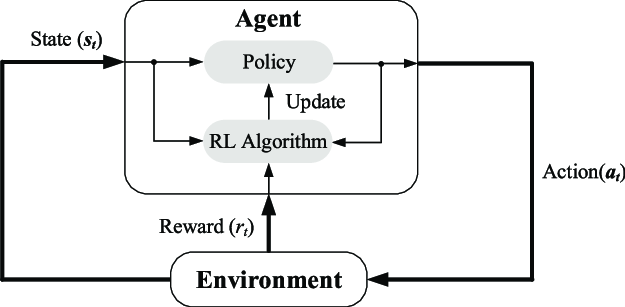
\includegraphics[width=0.8\textwidth]{figs/esquemaRL.png}
	\caption{Esquema d'interacció en el DRL \cite{esquemaRL}.}
	\label{fig:context-anoni1}
\end{figure}


Matemàticament, aquest problema es pot descriure mitjançant un procés de decisió de Markov, definit per $\langle \mathcal{S}, \mathcal{A}, p, r, \gamma\rangle$ \cite{DRLIntro}. El conjunt $\mathcal{S}$ representa els \emph{estats} possibles de l'entorn; $\mathcal{A}$ és el conjunt d'accions disponibles; $p(s' \mid s,a)$ és la probabilitat de transitar a l'estat $s'$ en executar l'acció $a$ a l'estat $s$; $r(s,a)$ defineix la recompensa obtinguda i $\gamma \in [0,1]$ és el factor de descompte que pondera les recompenses futures. A cada pas de temps $t$, l'agent observa un estat $s_t$, tria una acció $a_t$ i rep una recompensa $r_t$ \cite{RLIntro}. L'objectiu final és maximitzar la suma de recompenses futures (retorn), expressada sovint com :

\begin{equation}
G_t \;=\; \sum_{k=0}^{\infty} \,\gamma^k \, r_{t+k+1}.
\end{equation}

\paragraph{Actors principals: agent, entorn, estat i acció}

\begin{itemize}
\item \textbf{Agent}: És el sistema que pren decisions a cada pas. L'agent manté o aprèn una estratègia, anomenada \emph{política} $\pi(a \mid s)$, que determina amb quina probabilitat triarà cada acció $a$ si es troba a l'estat $s$ \cite{M1}.

\item \textbf{Entorn}: És el medi extern on l'agent actua. Rep l'acció de l'agent i actualitza l'estat, retornant la nova observació $s_{t+1}$ i la recompensa $r_{t+1}$ \cite{M1}. L'entorn pot ser complex i contenir característiques molt variades, incloses dades numèriques i dades qualitatives provinents de fonts no estructurades, com poden ser les notícies .

\item \textbf{Estat} ($s \in \mathcal{S}$): La informació rellevant del medi en un instant concret. Quan és tracta d'un sistema de Markov, es considera que $s$ conté tota la informació necessària per decidir l'acció òptima, sense haver de dependre de tots els estats previs \cite{M1}.

\item \textbf{Acció} ($a \in \mathcal{A}$): La decisió que pren l'agent en un estat determinat, com ara “comprar”, “vendre” o “mantenir” en un mercat financer \cite{M1}.
\end{itemize}

\paragraph{Funcions de valor i política}

En aprenentatge per reforç, l'agent aprèn funcions de valor per estimar la qualitat dels estats o de les accions. La funció de valor d'estat, $V^\pi(s)$, mesura el retorn esperat en trobar-se a l'estat $s$ i seguir la política $\pi$. De manera anàloga, la funció de valor d'acció, $Q^\pi(s,a)$, mesura el retorn esperat de prendre l'acció $a$ a l'estat $s$ i continuar amb la política $\pi$. Formalment \cite{M1}:

\begin{equation}
V^\pi(s) \;=\; \mathbb{E}_\pi\bigl[G_t \,\big\vert\, s_t = s\bigr]
\end{equation}
\begin{equation}
Q^\pi(s,a) \;=\; \mathbb{E}_\pi\bigl[G_t \,\big\vert\, s_t = s,\; a_t = a\bigr].
\end{equation}

La \textbf{política} òptima $\pi^*$ és aquella que maximitza el retorn acumulat; sovint, però, s'aprèn mitjançant aproximacions successives fins a trobar un bon resultat. Quan els espais d'estats o d'accions són molt grans, s'utilitzsen xarxes neuronals profundes per aproximar $Q$ o $V$ de manera eficient \cite{RLIntro}.

\vspace{2ex}
Dins d'aquest marc general, en el DRL s'han proposat diversos mètodes que resolen el problema de presa de decisions sota diferents estratègies de modelatge i optimització. A continuació, es descriuen els tres mètodes que s'han considerat en aquest treball.

\subsubsection{Deep Q-Network (DQN)}

El mètode Deep Q-Network (DQN) és un dels pilars fonamentals de l'aprenentatge per reforç profund (DRL), i representa l'aplicació directa de xarxes neuronals profundes per aproximar la funció d'acció-valor $Q(s, a)$ pròpia del mètode Q-learning. La seva introducció per DeepMind \cite{MnihNature2015} va marcar un abans i un després, aconseguint un rendiment superior al de humans en diversos jocs d'Atari \cite{M9}.

\paragraph{Q-learning revisat:}
El Q-learning és un algorisme de control off-policy que permet aprendre una política òptima mitjançant la maximització del valor esperat del retorn acumulat. La funció de valor $Q$ s'actualitza iterativament a partir de l'experiència de l'agent, segons la següent equació:

\begin{equation}
Q(s_t, a_t) \leftarrow Q(s_t, a_t) + \alpha \left[ r_{t+1} + \gamma \max_{a'} Q(s_{t+1}, a') - Q(s_t, a_t) \right]
\end{equation}

En aquest cas, $\alpha$ representa la taxa d'aprenentatge, $r_{t+1}$ és la recompensa obtinguda després de realitzar l'acció $a_t$ en l'estat $s_t$, i $\gamma$ és el factor de descompte que pondera les recompenses futures. L'objectiu és refinar progressivament l'estimació de $Q(s,a)$ per reflectir millor els guanys a llarg termini que pot aconseguir l'agent seguint una política determinada.

Tot i la seva eficàcia en entorns simples, Q-learning té moltes limitacions quan s'aplica a espais d'estats molt grans o continus. En aquests casos, l'agent no pot utilitzar una taula explícita $Q(s,a)$ a causa de les limitacions de memòria i de l'eficiència computacional. Per sol·lucionar això, va sorgir l'algorisme Deep Q-Network (DQN), que substitueix la taula Q per una xarxa neuronal que aproxima la funció $Q(s,a)$ a través de paràmetres ajustables $\theta$, de manera que $Q(s,a; \theta) \approx Q^*(s,a)$.


\paragraph{Arquitectura DQN:}

L'arquitectura d'una DQN es basa en una xarxa neuronal profunda, que pot modificar-se segons la naturalesa de les dades d'entrada. Quan es treballa amb imatges, per exemple, és habitual l'ús de xarxes convolucionals (CNN); en altres contextos, poden emprar-se arquitectures totalment connectades o específiques del domini. La sortida de la xarxa és un vector que conté els valors Q estimats per a cada acció possible a partir d'un estat donat.


\paragraph{Funció de pèrdua i entrenament:}

L'aprenentatge de la DQN es basa en la minimització de la diferència entre la predicció de la xarxa i un valor objectiu $y_t$, derivat de la fórmula de Bellman. La funció de pèrdua que s'utilitza habitualment és:

\begin{equation}
\mathcal{L}(\theta) = \mathbb{E}_{(s,a,r,s') \sim \mathcal{D}} \left[ \left( y_t - Q(s, a; \theta) \right)^2 \right]
\end{equation}

on el valor objectiu es calcula com $y_t = r + \gamma \max_{a'} Q(s', a'; \theta^-)$, i $\theta^-$ representa els pesos d'una còpia fixa de la xarxa principal (target network) que s'actualitza periòdicament.


\paragraph{Tècniques per estabilitzar DQN:}
Per garantir un entrenament estable i eficient, DQN implementa diverses estratègies. La primera és l'ús d'una target network, una rèplica de la xarxa principal amb pesos congelats durant un cert nombre d'iteracions, que s'utilitza per calcular els valors objectiu $y_t$ de manera més robusta. La segona és l'\textit{experience replay}, que consisteix a emmagatzemar les transicions $(s,a,r,s')$ en una memòria i mostrejar-les aleatòriament durant l'entrenament. Això trenca la correlació temporal entre les mostres i millora l'eficiència del procés d'aprenentatge. Finalment, per garantir un equilibri entre exploració i explotació, s'adopta una política $\varepsilon$-greedy, en què l'agent selecciona accions aleatòries amb una probabilitat $\varepsilon$, afavorint l'exploració durant l'entrenament \cite{M9}\cite{MnihNature2015}.


\subsubsection{Proximal Policy Optimization (PPO)}

El mètode Proximal Policy Optimization (PPO) és un dels algorismes d'aprenentatge per reforç profund més utilitzats actualment. Va ser proposat per OpenAI com una alternativa robusta i eficient als mètodes de gradient de política tradicionals com REINFORCE o TRPO (Trust Region Policy Optimization)\cite{schulman2017}. Es caracteritza per combinar estabilitat, eficiència en el càlcul i ser fàcilment implementable.


Es tracta d'un mètode basat en gradient de política (PG). Aquests mètodes actualitzen els paràmetres de la política directament segons:

\begin{equation}
\theta_{t+1} \leftarrow \theta_t + \alpha \nabla_\theta J(\theta)
\end{equation}

on $J(\theta)$ és una estimació del retorn esperat. Tanmateix, actualitzacions massa grans poden trencar la política i provocar divergències. PPO simplifica aquesta idea limitant els canvis de política mitjançant una funció de pèrdua acotada.

L'objectiu de PPO és maximitzar el \textit{clipped surrogate objective}, que segueix la següent expressió:

\begin{equation}
\mathcal{L}^{\text{CLIP}}(\theta) = \mathbb{E}_t \left[ \min \left( r_t(\theta) \hat{A}_t, \, \text{clip}(r_t(\theta), 1 - \epsilon, 1 + \epsilon) \hat{A}_t \right) \right]
\end{equation}

on $r_t(\theta) = \frac{\pi_\theta(a_t | s_t)}{\pi_{\theta_{\text{old}}}(a_t | s_t)}$ és el quocient entre la nova política i la política antiga, i $\hat{A}_t$ és l'avantatge estimat en el temps $t$, generalment calculat com $\hat{A}_t = Q(s_t,a_t) - V(s_t)$. El paràmetre $\epsilon$, típicament entre 0.1 i 0.3, controla la tolerància als canvis. Si $r_t$ surt dels límits establerts, l'actualització queda truncada i no rep recompensa addicional, evitant així desviacions molt brusques.

\paragraph{Estimació de l'avantatge:}
Per reduir la variància en l'estimació de l'avantatge s'utilitza sovint el mètode \textbf{GAE (Generalized Advantage Estimation)}:

\begin{equation}
\hat{A}_t = \sum_{l=0}^{\infty} (\gamma \lambda)^l \delta_{t+l}
\end{equation}

on $\delta_t = r_t + \gamma V(s_{t+1}) - V(s_t)$ i $\lambda$ és un hiperparàmetre que regula el compromís entre biaix i variància. Aquesta estimació suavitza l'avantatge i contribueix a millorar la qualitat dels gradients.


El funcionament complet de PPO es pot resumir en les següents etapes, repetides a cada iteració d'entrenament:
\begin{enumerate}
  \item Es recullen trajectòries executades per la política actual $\pi_\theta$.
  \item Es calculen els valors de retorn, la funció de valor $V(s)$ i l'avantatge $\hat{A}_t$.
  \item Es realitza l'entrenament durant diverses èpoques minimitzant $\mathcal{L}^{\text{CLIP}}(\theta)$, habitualment amb l'optimitzador Adam.
  \item Finalment, es copia la política actual per actualitzar la política antiga: $\theta_{\text{old}} \leftarrow \theta$.
\end{enumerate}


\subsubsection{Soft Actor-Critic (SAC)}

El Soft Actor-Critic (SAC) és un dels algorismes d'aprenentatge per reforç profund més eficients dissenyat per operar en entorns amb espais d'accions continus \cite{Haarnoja2018}. Forma part dels mètodes \textit{actor-crític off-policy}, però amb la novetat que a banda d'optimitzar el retorn esperat, també maximitza l'entropia de la política, afavorint polítiques més deterministes i exploratòries \cite{M11}.

A diferència d'altres enfocaments que busquen únicament maximitzar la recompensa, el SAC té dos objectius. D'una banda, vol obtenir un retorn acumulat elevat; de l'altra, manté l'entropia de la política elevada per evitar una convergència prematura cap a solucions deterministes. Aquest objectiu es tradueix en la següent expressió:

En lloc de maximitzar només el retorn esperat acumulat, SAC maximitza l'objectiu següent:

\begin{equation}
J(\pi) = \mathbb{E}_{\tau \sim \pi} \left[ \sum_t r(s_t, a_t) + \alpha \mathcal{H}(\pi(\cdot|s_t)) \right]
\end{equation}

Aquí, $\mathcal{H}$ és l'entropia de la política, i $\alpha$ és un hiperparàmetre que controla el pes assignat al terme d'exploració. Com més alt sigui $\alpha$, més probabilitat tindrà l'agent de mantenir accions aleatòries, evitant una convergència massa ràpida.

\paragraph{Arquitectura del SAC:}

L'arquitectura del SAC integra diversos components que treballen conjuntament. El primer és l'actor $\pi_\phi(a|s)$, una política estocàstica que genera accions a partir d'una distribució probabilística —habitualment una gaussiana parametritzada. El segon són dos crítics, $Q_{\theta_1}(s,a)$ i $Q_{\theta_2}(s,a)$, que proporcionen estimacions de valor independents. Aquest disseny amb doble crític busca reduir el biaix per sobreaprenentatge, prenent el mínim dels dos valors en les actualitzacions. Finalment, també s'incorporen versions retardades dels crítics, conegudes com a \textit{target critics}, que s'usen per millorar l'estabilitat del procés d'entrenament.


L'entrenament del SAC gira al voltant de tres funcions d'objectiu diferenciades. En primer lloc, els crítics s'actualitzen per mitjà de l'error de temporal difference (TD), fent servir una estimació suau del retorn que inclou el terme d'entropia de la política:
  \begin{equation}
  y(r,s') = r + \gamma \left( \min_{i=1,2} Q_{\theta'_i}(s', a') - \alpha \log \pi_\phi(a'|s') \right)
  \end{equation}

  En segon lloc, l'actor es millora mitjançant la minimització d'una pèrdua que combina el valor esperat negatiu amb el terme d'entropia, afavorint aquelles accions que siguin valuoses i exploratòries alhora:

  \begin{equation}
  \mathcal{L}_{\text{actor}} = \mathbb{E}_{s_t \sim \mathcal{D}} \left[ \alpha \log \pi_\phi(a_t|s_t) - Q_{\theta}(s_t, a_t) \right]
  \end{equation}

  Finalment, l'hiperparàmetre $\alpha$, que controla el pes del terme d'entropia, pot ajustar-se automàticament durant l'entrenament. Aquesta adaptació es fa mitjançant l'optimització d'una tercera funció de pèrdua:

  \begin{equation}
  \mathcal{L}(\alpha) = \mathbb{E}_{a_t \sim \pi} \left[ -\alpha \log \pi(a_t|s_t) - \alpha \mathcal{H}_\text{target} \right]
  \end{equation}


Gràcies a aquests elements, SAC és molt robust i eficient. El seu enfocament off-policy permet aprofitar dades acumulades en experiències passades, fet que incrementa l'eficiència. Alhora, la regularització mitjançant entropia manté una exploració activa i sostinguda durant l'entrenament. L'ús de dues xarxes Q redueix significativament el biaix en les estimacions de valor, i l'ajust automàtic del paràmetre $\alpha$ facilita un equilibri dinàmic entre exploració i explotació \cite{Haarnoja2018}.

\vspace{2em}

Per tal de sintetitzar les diferències i similituds entre els algorismes d'aprenentatge per reforç profund analitzats, es presenta la següent taula comparativa.
\begin{table}[h]
\centering
\caption{Comparativa dels algoritmes de DRL utilitzats}
\begin{tabular}{lccc}
\hline
\textbf{Característica} & \textbf{DQN} & \textbf{PPO} & \textbf{SAC} \\ \hline
Tipus & Basat en valor & Basat en política & Actor-Crític \\
Espai d'accions & Discret & Discret/Continu & Continu \\
Exploració & $\epsilon$-greedy & Clipping gradient + GAE & Maximització entropia \\
Replay buffer & Sí & No & Sí \\
Estabilitat & Moderada & Alta & Alta \\ \hline
\end{tabular}
\label{tab:comparativa_algoritmes}
\end{table}



\subsection{Natural language processing}

 Les tècniques de Processament del Llenguatge Natural permeten extreure característiques clau dels textos, ja sigui en forma de paraules rellevants, temàtiques predominants o sentiments. A continuació es descriuen les tècniques que s'han considerat en aquest treball.

\subsubsection{Word2Vec}

Word2Vec és una tècnica d'aprenentatge no supervisat que permet transformar paraules en vectors numèrics amb dimensió fixa, capturant relacions semàntiques entre mots a partir del seu context \cite{Mikolov2013}. A diferència de representacions basades en freqüències, com TF-IDF, Word2Vec aprèn aquestes representacions mitjançant una xarxa neuronal entrenada sobre seqüències de text, de manera que paraules amb usos similars es representen per vectors propers en l'espai.

Hi ha dues arquitectures principals per entrenar Word2Vec:

\begin{itemize}
    \item \textbf{Continuous Bag-of-Words (CBOW):} prediu una paraula a partir del seu context (les paraules del voltant).
    \item \textbf{Skip-gram:} fa la tasca inversa: prediu el context a partir d'una sola paraula.
\end{itemize}

El model genera, per a cada paraula, un vector numèric de longitud $d$ que resumeix la seva relació amb altres paraules segons l'ús en el text. Per tant, paraules que apareixen en contextos similars acaben tenint vectors propers en l'espai.

Per obtenir una representació vectorial d'un text com pot ser un conjunt de notícies, és habitual calcular la mitjana dels vectors de totes les paraules que el componen. Això proporciona una única representació densa que resumeix el contingut global del text.

En aquest projecte s'utilitza la variant \texttt{Skip-gram}, ja que funciona millor per a textos amb molta informació, com pot ser el cas de notícies.

Aquesta representació forma part de l'observable per l'agent d'aprenentatge per reforç.


\subsubsection{Topic Modeling (LDA)}

El \emph{Topic Modeling} busca descobrir temàtiques latents en un conjunt de documents de manera no supervisada. Latent Dirichlet Allocation (LDA) és un dels models més populars \cite{Blei2003}. LDA assumeix que:

\begin{itemize}
\item Cada document és una barreja de temes en diferents proporcions.
\item Cada tema és una distribució de probabilitat sobre el vocabulari.
\end{itemize}

Formalment, si es tenen $K$ temes i $D$ documents, LDA estima distribucions $\theta_d$ (barreges de temes del document $d$) i $\phi_k$ (distribució de paraules del tema $k$). En aquest cas, un cop inferit, es pot assignar a cada notícia la probabilitat de pertànyer a cada tema, creant un vector de característiques que es pot incorporar a l'estat de l'agent.

\begin{figure}[H]
	\centering
	\includegraphics[width=0.8\textwidth]{figs/tm.png}
	\caption{Esquema del funcionament del Topic Modeling\cite{esquemaRL}.}
	\label{fig:context-anoni1}
\end{figure}

\subsubsection{Anàlisi de sentiments}

L'anàlisi de sentiments pretén determinar la polaritat (positiva, negativa o neutra) d'un text \cite{kennedy2006sentiment}. Les tècniques més senzilles es basen en diccionaris de paraules amb connotació positiva o negativa, mentre que els mètodes avançats utilitzen models supervisats o xarxes neuronals de tipus \emph{Transformers} \cite{TABINDAKOKAB2022100157}. En l'àmbit financer, detectar ràpidament un sentiment negatiu pot anticipar vendes massives, mentre que un sentiment marcadament positiu pot indicar expectatives alcistes del mercat.


\subsection{Integració de NLP i DRL}

La utilització de tècniques NLP en agents DRL s'ha convertit en una possible estratègia per al desenvolupament de sistemes de trading algorítmic més informats i adaptatius. Aquesta combinació permet incorporar no només dades numèriques històriques com preus o volums, sinó també informació qualitativa provinent de diferents fonts, com ara notícies financeres o xarxes socials.

Tot i que la literatura en aquest àmbit no és extensa, hi ha publicacions que tracten aquest tema. Per exemple, en \cite{gangopadhyay}, es proposa un model DDPG (Deep Deterministic Policy Gradient) enriquit amb embeddings semàntics de notícies per millorar les decisions d'inversió. Els resultats mostren una millora significativa en el rendiment de l'algoritme d'inversió.

En un altre estudi rellevant és un treball de final de grau, \cite{alvarez2023real}, on s'utilitzen representacions BERT de notícies financeres en temps real combinades amb informació de mercat per alimentar un agent DRL. Aquest sistema demostra una millor capacitat d'anticipació de tendències respecte a models que només utilitzen dades numèriques.

A més, s'ha observat que la incorporació d'informació provinent de xarxes socials, com Twitter o Reddit, pot afegir valor predictiu. En \cite{DBLP}, es mostra com aquesta informació  pot millorar l'eficiència d'agents basats en DQN i PPO quan s'apliquen a mercats volàtils com el de les criptomonedes.




\chapter{Implementació}

En aquest capítol es descriu l'execució pràctica del treball, mostrant com s'han implementat els conceptes teòrics exposats en els capítols anteriors.

Primerament, s'explica l'obtenció i preprocessament de les dades, que inclou tant dades històriques de mercat com titulars de notícies econòmiques. Posteriorment, es descriu el tractament del llenguatge natural, on aquestes notícies es transformen en representacions vectorials mitjançant tècniques com la modelització de temes i l'anàlisi de sentiments.

El capítol segueix amb la creació de l'estat que rebrà l'agent en cada pas de temps, unint les característiques tècniques i les característiques semàntiques en un únic vector. Després es mostra com s'ha creat l'entorn de simulació desenvolupat amb OpenAI Gym, que simula l'evolució del mercat i permet als agents interactuar amb ell.

Seguidament, es presenten els tres agents implementats (DQN, PPO i SAC), les corresponents arquitectures, la configuració i el procés d'entrenament. Per últim, es descriu el procediment d'avaluació i comparació de resultats, utilitzant mètriques específiques per a analitzar el comportament dels agents.

\subsection{Arquitectura del projecte}
El projecte s'ha desenvolupat seguint una arquitectura modular basada en la separació de responsabilitats. Aquest codi inclou tot el flux del projecte, des de l'obtenció de les dades fins a l'execució dels agents. El repositori es divideix principalment en les següents carpetes:

\begin{itemize}
    \item \textbf{scripts/}: Conté els scripts d'execució independents que permeten executar el procés complet o parcial del projecte per facilitar la depuració del codi.
    \begin{itemize}
        \item \texttt{01-news\_extraction.py}: descarrega les notícies mensuals des de l'API del New York Times.
        \item \texttt{02-join\_news\_extraction.py}: concatena les notícies obtingudes en un únic fitxer i hi afegeix metadades.
        \item \texttt{03-news\_analysis.py}: filtra notícies repetides i selecciona les més rellevants per dia.
        \item \texttt{04-news\_cleaning.py}: neteja els textos, elimina soroll i assigna la data efectiva de mercat a cada notícia.
        \item \texttt{05-natural\_language\_processing.py}: aplica tècniques NLP (Word2Vec, LDA, FinBERT) per obtenir un vector numèric a partir de les notícies.
        \item \texttt{06-market\_data.py}: descarrega dades històriques dels actius (SPY, USO) i calcula indicadors tècnics.
        \item \texttt{07-state\_builder.py}: fusiona les dades quantitatives i qualitatives per construir els estats d'entrada de l'agent.
        \item \texttt{08-dqn\_with\_news.py}, \texttt{09-ppo\_with\_news.py}, \texttt{10-sac\_with\_news.py}: entrenen els agents DQN, PPO i SAC amb notícies com a part de l'estat.
        \item \texttt{11-dqn\_without\_news.py}, \texttt{12-ppo\_without\_news.py}, \texttt{13-sac\_without\_news.py}: entrenen els però sense informació qualitativa (només dades de mercat).
        \item \texttt{14-results.py}: recull i visualitza els resultats obtinguts.
    \end{itemize}

    \item \textbf{data/}: directori destinat a les dades d'entrada i sortida del projecte. S'organitza en:
    \begin{itemize}
        \item \texttt{raw/}: conté les dades tal com s'obtenen de les fonts originals (API i llibreria de yfinance).
        \item \texttt{processed/}: conté fitxers ja netejats, vectors NLP, dades de mercat i estats fusionats.
        \item \texttt{models/}: conté els models entrenats i els corresponents logs.
        \item \texttt{results/}: conté els resultats i gràfiques dels models.
    \end{itemize}

    \item \textbf{src/news/}: inclou els mòduls relacionats amb l'obtenció i tractament de notícies.
    \begin{itemize}
        \item \texttt{extraction.py}: extracció de notícies des de l'API.
        \item \texttt{news\_processor.py}: generació del text complet i integració d'etiquetes.
        \item \texttt{nlp\_processor.py}: vectorització amb LDA, Word2Vec i anàlisi de sentiments.
        \item \texttt{text\_processor.py}: neteja lèxica i estructural de textos.
        \item \texttt{generate\_new\_date.py}: funció per a assignar la data a la notícia segons el mercat en el que s'opera.
    \end{itemize}

    \item \textbf{src/rl/}: Mòduls d'aprenentatge per reforç i entorn de simulació.
    \begin{itemize}
        \item \texttt{agents/}: implementació dels agents \texttt{DQN}, \texttt{PPO} i \texttt{SAC}, heretant d'un agent base\texttt{BaseAgent}.
        \item \texttt{state\_assembler.py}: construcció i normalització de l'estat complet de l'agent.
        \item \texttt{stock\_env.py}: implementació de l'entorn de trading amb OpenAI Gym.
    \end{itemize}

    \item \textbf{src/market/}: inclou els mòduls directament relacionats amb les dades de mercat.
    \begin{itemize}
        \item \texttt{market\_data\_extractor.py}: obtenció de dades de mercat i càlcul d'indicadors tècnics.
    \end{itemize}
\end{itemize}

\subsection{Obtenció i preprocessament de les dades}

Les dades utilitzades en aquest projecte provenen de dues fonts principals: notícies econòmiques de caràcter internacional i informació històrica de mercat.

\subsubsection{Obtenció de notícies}

Les notícies utilitzades en aquest projecte s'han obtingut a través de l'API pública del \textit{New York Times}, cobrint el període comprès entre gener de 2014 i abril de 2025. Per  a l'obtenció, s'ha fet una petició separada per a cada mes dins d'aquest interval. Això ha permès iterar sobre el període complet i, al mateix temps, respectar les limitacions de l'API de màximes sol·licituds per minut.

Per a cada notícia descarregada es recuperen diversos camps estructurats, dels quals s'han només conservat aquells més rellevants per als objectius d'aquest projecte. Concretament:

\begin{itemize}
    \item \textbf{Títol}: frase principal que sintetitza el contingut de la notícia (\texttt{headline.main}).
    \item \textbf{Resum}: breu descripció dels fets destacats, extreta del camp \texttt{snippet} o, si aquest no està disponible, de \texttt{abstract}.
    \item \textbf{URL}: enllaç directe a la notícia publicada en línia (\texttt{web\_url}).
    \item \textbf{Data de publicació}: data de publicació de l'article (\texttt{pub\_date}), necessària per sincronitzar cronològicament les notícies amb les dades de mercat.
    \item \textbf{Secció}: categoria principal assignada pel mitjà (\texttt{section\_name}) que indica l'àmbit temàtic general de la notícia.
    \item \textbf{Subsecció}: subcategoria dins la secció principal (\texttt{subsection\_name}) que afina la temàtica de l'article.
    \item \textbf{Mitjà de publicació}: font que ha publicat la notícia (\texttt{source}), generalment el mateix \textit{New York Times}.
    \item \textbf{Tipus de document}: classificació del contingut segons el tipus de contingut (\texttt{document\_type}), com per exemple “article” o “multimedia”.
    \item \textbf{Tipus de material}: indica el tipus de notícia (\texttt{type\_of\_material}), com ara “News”, “Op-Ed” o “Review”.
    \item \textbf{Identificador}: identificador intern únic (\texttt{new\_id}) assignat a cada notícia, utilitzat per relacionar-la amb les seves paraules clau corresponents.
    \item \textbf{Paraules clau}: conjunt d'etiquetes (\texttt{keywords}) associades a cada notícia, que identifiquen entitats, temes, persones o llocs esmentats. Cada paraula clau inclou el seu tipus (\texttt{name}), el valor concret (\texttt{value}) i la seva rellevància relativa (\texttt{rank}) dins la pròpia notícia.
\end{itemize}

D'aquest procés s'obtenen aproximadament 1.35 milions de notícies.

\begin{figure}[H]
	\centering
	\includegraphics[width=1\textwidth]{figs/top_sections_subsections.png}
	\caption{Distribució de noticies per seccions i subseccions}
	\label{fig:context-anoni1}
\end{figure}



\subsubsection*{Neteja i filtratge}

Un cop descarregades, les notícies es netegen i es filtren amb l'objectiu de garantir la qualitat del conjunt de dades i eliminar aquelles notícies que no són rellevants per a aquest cas.

En primer lloc, es descarten aquells articles que no disposen de camps essencials com el títol, el resum o la data de publicació.

Tot seguit, s'identifiquen casos de duplicació de contingut. És habitual que una mateixa notícia aparegui més d'una vegada amb petites variacions (canvis de secció, petites edicions en el títol, etc.). Per tractar aquest casos, es defineix una clau de duplicació basada en la data i el títol, i es conserva només la versió més recent de cada notícia.

Després d'aquesta primera neteja, s'aplica un filtratge segons el contingut per garantir que només es conserven notícies que puguin ser informatives per a un agent d'inversió. Aquest filtratge es duu a terme en tres nivells:

\begin{itemize}
    \item \textbf{Secció i subsecció}: només s'inclouen notícies publicades en seccions generals com \textit{World}, \textit{U.S.} o \textit{Business Day}, i en subseccions específiques com \textit{Economy}, \textit{Europe}, \textit{International Business} o \textit{Stocks and Bonds}. Aquestes àrees haurien de cobrir les temàtiques econòmiques, polítiques i corporatives son d'interes en aquest cas.

    \item \textbf{Tipus de document}: s'exclouen entrades que no siguin de tipus \texttt{article}. Aquesta condició assegura que només es treballa amb notícies completes i redactades amb finalitat informativa.

    \item \textbf{Tipus de material}: es manté només aquell contingut classificat com a \texttt{News} dins del camp \texttt{type\_of\_material}, descartant formats com “Op-Ed”, “Review” o “Obituary”, que no aporten valor informatiu en el context d'un model predictiu.
\end{itemize}

El resultat d'aquesta neteja són al voltant de 117 mil notícies, al voltant d'un 8\% de les notícies obtingudes de l'API.
\begin{figure}[H]
	\centering
	\includegraphics[width=0.8\textwidth]{figs/news_per_year.png}
	\caption{Distribució de les notícies resultants de la neteja i preprocessament per any.}
	\label{fig:context-anoni1}
\end{figure}

\subsubsection*{Assignació temporal i unificació de text}

Per garantir una alineació temporal rigorosa entre les notícies i les dades de mercat, s'ha definit per a cada article una data efectiva de mercat. Aquesta data representa el primer dia hàbil en què la notícia hauria pogut ser coneguda i processada pels inversors abans de l'obertura dels mercats.

Aquest pas es fa per evitar biaixos de futur, assegurant que cada decisió presa per l'agent només es basa en informació que hauria d'estar disponible en aquell moment del temps. El càlcul es realitza comprovant si la notícia ha estat publicada abans o després d'una hora límit, que en aquest cas és una hora abans de l'obertura del mercat en el que es treballa. En cas que la notícia arribi massa tard, la data efectiva és el següent dia hàbil.

Un cop assignada la data efectiva de mercat, es procedeix a unificar les diferents parts de la notícia en un únic text amb tota la informació. L'objectiu d'aquest pas és que cada notícia pugui ser processada com una única unitat semàntica. Per fer-ho, es construeix un nou camp anomenat \texttt{full\_text}, que concatena tres fonts d'informació: el títol, el resum (\texttt{snippet} o \texttt{abstract}) i les etiquetes semàntiques associades a l'article ordenades per rellevància.

El resultat és una cadena de text que representa tot el contingut de la notícia apta per ser processada amb NLP.


\subsubsection{Obtenció de dades de mercat}

Per tal de complementar les característiques qualitatives extretes de les notícies amb informació quantitativa, s'han seleccionat dos actius financers amb perfils diferenciats. Aquests actius permeten explorar si la incorporació de notícies aporta valor en entorns diferents, com ara tendències de mercat o situacions de crisi.

\begin{itemize}
    \item \textbf{SPY}: És l'ETF que replica l'evolució de l'índex S\&P 500, un dels principals indicadors del mercat borsari dels Estats Units. Aquest actiu representa el comportament agregat de grans empreses nord-americanes i és sensible a decisions econòmiques o canvis en la situació política, sobretot la dels Estats Units. El seu perfil respon a escenaris de creixement, volatilitat o estabilitat econòmica.

    \item \textbf{USO}: És l'ETF que replica l'evolució del preu del petroli cru dels Estats Units. Es tracta d'un actiu altament sensible a esdeveniments geopolítics i econòmics, com sancions internacionals o conflictes en regions productores de petroli. Aquest tipus d'esdeveniments tenen una cobertura mediàtica molt extensa i de manera pràcticament immediata, això fa del petroli pugui ser un actiu especialment interessant per avaluar si l'agent és capaç relacionar aquest tipus de notícies amb el preu d'aquest EFT.

\end{itemize}

L'històric de dades d'aquests actius s'han obtingut a través de la llibreria \texttt{yfinance}, que proporciona accés a dades de mercat diàries de fonts com Yahoo Finance. Per a cada actiu s'han descarregat els preus d'obertura, màxim, mínim, tancament, volum i identificador del ticker. El període analitzat comprèn des de gener de 2014 fins a abril de 2025, afegint un marge de 60 dies anteriors per a poder fer el càlcul d'indicadors tècnics a partir de l'1 de gener de 2014.

\subsubsection*{Càlcul d'indicadors tècnics}

A banda del preu dels actius, s'han calculat diversos indicadors tècnics a partir de les dades històriques de preus. Aquests indicadors són utilitzats habitualment en l'anàlisi de mercats financers per identificar tendències, moments d'entrada o sortida, i situacions de sobrecompra o sobrevenda.

Els indicadors s'han calculat amb la llibreria de Python \texttt{ta}. A partir dels preus de tancament i, en alguns casos, del volum, s'han afegit al conjunt de dades els següents indicadors:

\begin{itemize}
    \item \textbf{SMA (Simple Moving Average)}: la mitjana mòbil simple de 20 dies proporciona una visió suavitzada de la tendència recent del preu. Permet reduir el soroll de la sèrie temporal i identificar canvis de direcció amb menys volatilitat.

    \item \textbf{RSI (Relative Strength Index)}: indicador de momentum calculat sobre 14 períodes, que mesura la força relativa dels moviments positius i negatius del preu. Valors alts (per sobre de 70) poden indicar una situació de sobrecompra, mentre que valors baixos (per sota de 30) poden suggerir una situació de sobrevenda.

    \item \textbf{MACD (Moving Average Convergence Divergence)}: indicador de tendència basat en la diferència entre dues mitjanes mòbils exponencials (EMAs de 12 i 26 períodes), juntament amb una línia senyal (EMA de 9 períodes). Permet detectar possibles punts d'inflexió en el comportament del preu i generar senyals d'entrada o sortida.
\end{itemize}

Un cop calculats, aquests indicadors s'afegeixen com a noves columnes al conjunt de dades de mercat. Finalment, s'eliminen les files amb valors nuls resultants del càlcul (corresponents als primers 60 dies previs al gener de 2014).

\subsection{Processament del llenguatge natural}

L'objectiu del processament de notícies és convertir el conjunt de textos disponibles cada dia en un únic vector. Aquesta representació ha de ser prou compacta per ser integrable amb les dades de mercat, però també ha de capturar el context qualitatiu que pot influir en la dinàmica dels preus.

Cada dia es publiquen múltiples notícies, però per al nostre model, es busca obtenir un únic vector per jornada, de manera que l'estat de l'agent mantingui una estructura alineada amb les dades quantitatives. Hi ha diverses estratègies possibles per combinar múltiples textos en una sola representació, però en aquest projecte s'ha optat per seleccionar només les notícies que presenten un to emocional més extrem, assumint que aquestes tenen un impacte més directe en el mercat.

Aquest pipeline es pot dividir en quatre fases principals: anàlisi de sentiments, selecció de notícies, construcció del text agregat i extracció de característiques.

\subsubsection{Anàlisi de sentiments i selecció de notícies rellevants}

Per a cada dia, s'avalua la polaritat emocional de totes les notícies disponibles per a poder identificar les més rellevants. En un inici, es va considerar l'ús de la llibreria \texttt{TextBlob}, habitual en tasques d'anàlisi de sentiments però, es va observar que aquesta eina, pensada per a llenguatge general, no capturava correctament la rellevància o el context de notícies econòmiques i financeres.

Per aquest motiu, s'ha optat per \texttt{FinBERT}, un model basat en un Transformador i entrenat específicament sobre textos del domini financer.

La puntuació de sentiment retornada per FinBERT és un valor escalar entre -1 i +1, que expressa la polaritat general del text. A partir d'aquestes puntuacions, es calcula el valor absolut de cada notícia per mesurar-ne la intensitat emocional, i es seleccionen les 5 notícies més extremes (positives o negatives). Aquesta selecció de notícies es basa en la hipòtesi que aquestes notícies són també les que tenen més probabilitat d'influir en els moviments del mercat.


\subsubsection{Construcció i ús del text per al NLP}

Un cop identificades les notícies més rellevants, es concatenen en una única cadena de text. Aquesta agregació busca resumir el context informatiu dominant del dia en un text apte per al NLP.

Aquest text concatenat s'utilitza com a entrada principal per al pipeline de transformació, però no de la mateixa manera per a totes les tècniques, els canvis que rep aquest text són diferents segons les necessitats de cada procés.

\subsubsection{Preprocessament per a models semàntics}

Per a les tècniques Word2Vec i LDA, el text concatenat es neteja mitjançant el mòdul \texttt{TextProcessor}, que aplica:

\begin{itemize}
    \item Conversió a minúscules.
    \item Eliminació de caràcters especials, símbols i puntuació.
    \item Eliminació de nombres.
    \item Tokenització: divisió del text en paraules (tokens).
    \item Eliminació de paraules buides (\textit{stopwords}).
    \item Lematització: reducció de les paraules a la seva forma base.
\end{itemize}

Aquest text net resultant s'anomena \texttt{clean\_text} i és la base per a les tècniques de vectorització següents.

\subsubsection{Model Word2Vec}

El model Word2Vec s'utilitza per generar una representació semàntica del contingut informatiu rellevant de cada dia. Tant l'entrenament com l'aplicació es realitzen a partir del text netejat i concatenat de les notícies més destacades.

\paragraph{Entrenament}

El model s'entrena a partir dels textos prèviament netejats. Cada document es transforma en una seqüència de paraules, que s'utilitzen per entrenar el model mitjançant la implementació \texttt{Word2Vec} de la llibreria Gensim.

Els paràmetres emprats en l'entrenament són els següents:
\begin{itemize}
    \item \texttt{vector\_size} = 100: dimensió del vector que representa cada paraula.
    \item \texttt{window} = 5: mida de la finestra de context.
    \item \texttt{min\_count} = 3: només es tenen en compte paraules amb almenys 3 aparicions.
    \item \texttt{workers} = 8: nombre de fils de càlcul paral·lel.
\end{itemize}

El model s'entrena únicament sobre notícies publicades abans d'una data de tall determinada, que coincideix amb la data d'entrenament dels agents. Un cop entrenat, es desa per poder aplicar-lo a continuació.

\paragraph{Aplicació}

Per a cada dia, es tokenitza el text i, per a cada paraula, es comprova si existeix al vocabulari del model. Si és així, es recupera el seu vector corresponent. La mitjana de tots aquests vectors forma el vector semàntic del dia, una única representació de dimensió 100 que resumeix el significat general de les notícies del dia. Aquest vector forma part de l'estat observat per l'agent d'aprenentatge per reforç.

\vspace{1em}

\subsubsection{Model LDA}

El model LDA (Latent Dirichlet Allocation) s'utilitza per capturar la distribució temàtica del contingut de notícies de cada dia.

\paragraph{Entrenament}

L'entrenament del model es fa també sobre notícies anteriors a una data de tall, utilitzant el text net prèviament processat. Primer es construeix una matriu document-terme mitjançant \texttt{CountVectorizer}, que filtra paraules amb poca freqüència per reduir el soroll (\texttt{min\_df} = 5). Aquesta matriu representa cada dia com un vector de freqüències de paraules.

El model LDA s'entrena sobre aquesta matriu i infereix un conjunt de 10 temes. Cada tema s'identifica per un conjunt de paraules representatives, i el model aprèn una distribució de probabilitat per a cada document sobre aquests temes.


\paragraph{Aplicació}

S'aplica el model LDA entrenat per obtenir un vector de probabilitats de longitud $k=10$, que reflecteix la proporció en què cada tema és present en el conjunt informatiu del dia. A l'igual que en el cas del Word2Vec, aquest vector també forma part de l'estat d'entrada de l'agent.


\subsubsection{Tractament del sentiment}

Per calcular el valor del sentiment global del dia, s'utilitza el text concatenat original, sense aplicar-hi preprocessament. FinBERT ha estat entrenat amb text natural, i netejar-lo pot eliminar informació rellevant.

A partir d'aquest text i de les notícies més rellevants del dia, es calculen tres mètriques de sentiment:

\begin{itemize}
    \item \textbf{Sentiment global del dia}: valor entre -1 i +1 obtingut aplicant FinBERT sobre el text complet concatenat.
    \item \textbf{Mitjana del sentiment}: mitjana aritmètica de les notícies més rellevants.
    \item \textbf{Sentiment màxim}: valor de sentiment més positiu entre les notícies.
    \item \textbf{Sentiment mínim}: valor de sentiment més negatiu entre les notícies.
\end{itemize}

Finalment, el resultat final d'aquest NLP és una única fila per dia que conté:

\begin{itemize}
    \item \textbf{Data}: no s'inclou com a entrada per a l'agent, però és necessària per alinear les variables qualitatives i quantitatives.

    \item \textbf{Text complet concatenat}: tampoc s'inclou com a entrada, però serveix per verificar els resultats obtinguts o fer anàlisi qualitativa.

    \item \textbf{Vector semàntic mitjà} obtingut amb Word2Vec: vector de dimensió $d=100$, resultat de la mitjana dels vectors de paraula de les notícies del dia.

    \item \textbf{Vector temàtic} retornat per LDA: vector de probabilitats de dimensió $k=10$, que representa la presència relativa de cada tema.

    \item \textbf{Sentiment global del dia}: valor entre -1 i +1 obtingut per FinBERT aplicat al text concatenat.

    \item \textbf{Mitjana del sentiment}: mitjana aritmètica de les puntuacions individuals.

    \item \textbf{Sentiment màxim}: valor més positiu entre totes les notícies del dia.

    \item \textbf{Sentiment mínim}: valor més negatiu entre totes les notícies del dia.
\end{itemize}

Aquest vector representa la part qualitativa de l'estat que l'agent d'aprenentatge per reforç observarà en cada pas.

\subsection{Construcció de l'estat}

L'objectiu d'aquesta etapa és unir les característiques qualitatives derivades del processament de notícies amb les variables quantitatives provinents del mercat per formar un únic vector d'estat que l'agent pugui revisar durant la seva execució.

\subsubsection{Normalització de dades quantitatives}
En primer lloc, s'apliquen tècniques de normalització sobre els indicadors tècnics de mercat. El model utilitza un subconjunt seleccionat de variables: SMA, l'índex de força relativa RSI i l'indicador MACD. Aquestes variables s'estandarditzen mitjançant un \texttt{StandardScaler}, per evitar efectes associats a que les dades estiguin en diferents escales.

\subsubsection{Fusió amb les característiques qualitatives}

Un cop normalitzades les dades de mercat, es fa la fusió amb les dades qualitatives procedents del processament NLP. Aquesta unió es fa a través de la data de notícies, ja corregida prèviament, amb la data corresponent a valors quantitatius.


El resultat final és un dataframe on cada fila representa tota la informació diària única per a un actiu concret. Inclou:
\begin{itemize}
    \item Les característiques de mercat (preus, volum, indicadors tècnics normalitzats).
    \item Les característiques qualitatives per dia (Word2Vec, LDA, sentiment).
    \item La variable \texttt{ticker}, que permet identificar l'actiu.
    \item La data, que no serà utilitzada per l'agent però que permet ordenar les dades.
\end{itemize}

\subsection{Definició de l'entorn}
L'entorn de simulació utilitzat per entrenar els agents es basa en la llibreria \texttt{Gymnasium} i ha estat desenvolupat específicament per a tractar les característiques d'aquest treball. Aquest entorn reprodueix un mercat financer fictici on l'agent pot operar diàriament amb un actius, prenent decisions de compra o venda en funció d'un estat observat que inclou tant dades quantitatives com qualitatives.

\subsubsection{Espai d'estats}

L'estat observat en cada pas temporal està format per:
\begin{itemize}
    \item Les característiques del dia anterior (\texttt{d-1}) de l'actiu: indicadors tècnics, preus i dades de volum.
    \item Les característiques qualitatives de les notícies fins al moment de apertura del mercat, comunes a tots els actius: vector Word2Vec (dimensió 100), vector LDA (dimensió $k=10$) i sentiment (escala de -1 a 1).
    \item El diners restants actuals (\texttt{balance}) i el valor net de la cartera (\texttt{net\_worth}).
\end{itemize}

Tota aquesta informació s'afegeix en un vector d'observació.

\subsubsection{Espai d'accions}

L'entorn permet configurar dos tipus d'espai d'accions, seleccionables segons l'agent:
\begin{itemize}
    \item \textbf{Espai d'accions discret}: en aquest mode, l'agent disposa d'un conjunt finit de 7 accions possibles per a cada cada pas de temps. Aquestes accions són:
    \begin{itemize}
        \item \texttt{0}. No fer res.
        \item \texttt{1}. Comprar el 25\% del capital disponible.
        \item \texttt{2}. Comprar el 50\% del capital disponible.
        \item \texttt{3}. Comprar el 100\% del capital disponible.
        \item \texttt{4}. Vendre el 25\% de les accions en cartera.
        \item \texttt{5}. Vendre el 50\% de les accions en cartera.
        \item \texttt{6}. Vendre el 100\% de les accions en cartera.
    \end{itemize}

    \item \textbf{Espai d'accions continu}: en aquest mode, l'agent retorna un valor real entre -1 i 1. Aquest valor representa una acció contínua:
    \begin{itemize}
        \item Valors positius indiquen una compra. Per exemple, un valor de 0.6 implica comprar el nombre d'accions que pugui amb el 60\% del capital disponible.
        \item Valors negatius indiquen una venda. Per exemple, un valor de -0.4 implica vendre el 40\% de les accions en possessió.
        \item El valor 0 correspon a no operar.
    \end{itemize}
    Aquest espai és apte per l'agent SAC, que està dissenyat per a treballar en espais d'accions contínues.
\end{itemize}

\subsubsection{Funció de recompensa}

La funció de recompensa determina l'objectiu que l'agent intenta optimitzar. En aquest cas, s'ha definit com la variació relativa del valor net de la cartera entre dos dies consecutius:

\begin{equation}
r_t = \frac{\text{net\_worth}_t - \text{net\_worth}_{t-1}}{\text{net\_worth}_{t-1}} \cdot 100
\end{equation}

El valor net de la cartera (\texttt{net\_worth}) es calcula com la suma de l'efectiu disponible i el valor de mercat de totes les accions en propietat:

\begin{equation}
\text{net\_worth}_t = \text{cash}_t + \sum_{i=1}^{N} \left( \text{n\_shares}_i \cdot \text{price}_i \right)
\end{equation}

on:
\begin{itemize}
    \item cash és el capital no invertit disponible.
    \item n\_shares indica la quantitat d'accions en possessió per a cada actiu.
    \item price és el preu de tancament de l'actiu en el dia t.
\end{itemize}

A més de la recompensa principal, s'han incorporat penalitzacions suaus per incentivar un comportament actiu en l'agent:

\begin{itemize}
    \item \textbf{Accions inefectives}: si l'agent intenta comprar sense tenir diners o vendre sense tenir accions, es penalitza la recompensa.
    \item \textbf{Inacció prolongada}: si l'agent no compra ni ven durant més de 10 passos consecutius, s'aplica una penalització a la recompensa.
    \item \textbf{Estabilitat de capital durant la fase d'entrenament}: es penalitzen també els canvis mínims en el valor net (inferiors al 0.05\%), per evitar que l'agent opti per una estratègia massa conservadora o inactiva.
\end{itemize}

Aquestes recompenses i penalitzacions pretenen que l'agent tingui comportaments proactius alhora que incentiven l'augment de riquesa i penalitzen les pèrdues.

\subsubsection*{Condició de fallida}

Per evitar que l'agent segueixi estratègies massa especulatives, s'ha definit una condició de finalització anticipada si el valor net de l'agent cau per sota d'un 15\% del seu capital inicial.

\subsubsection{Mecàniques de cada pas}

L'agent pren les decisions basant-se en la informació disponible abans de l'obertura del mercat. De manera que, l'observable que s'utilitza per generar l'estat és el preu de tancament del dia anterior, simulant així el comportament d'un inversor que analitza el mercat amb dades del dia anterior. Tot i això, les accions que pren l'agent s'executen a partir del preu d'obertura del dia actual, tal com succeeix en un entorn real on les ordres es poden enviar abans que el mercat obri, però no s'executen fins que s'inicia la sessió.

El procés complet per a cada actiu en cada pas temporal segueix els passos següents:

\begin{enumerate}
    \item S'interpreta l'acció assignada per l'agent.
    \item Es calcula la quantitat a comprar o vendre tenint en compte el capital disponible o les accions en cartera, i es determina el cost de l'operació utilitzant el preu d'obertura del dia $t$.
    \item S'executa l'operació i s'actualitza l'estat intern de la cartera: saldo, nombre d'accions mantingudes i valor net total (\texttt{net\_worth}).
    \item Es registra tota la informació rellevant del pas: número d'iteració, data, accions realitzades, saldo, accions, valor net i recompensa.
    \item Finalment, es genera i retorna la nova observació de l'entorn, juntament amb la recompensa obtinguda i un indicador de finalització de l'episodi si escau.
\end{enumerate}


\subsection{Implementació dels agents}

En aquest projecte s'han implementat tres agents diferents: DQN, PPO i SAC. Cada un segueix un enfocament diferent, fet que permet comparar la seva capacitat per adaptar-se a l'entorn financer dissenyat. La implementació es basa en la llibreria \texttt{Stable-Baselines3}, i tots els agents comparteixen una interfície comuna definida a la classe \texttt{BaseAgent}, que gestiona l'entrenament i la validació.

Tots tres agents contenen paràmetres que defineixen el seu comportament. La selecció d'aquests es fa mitjançant l'optimització d'hiperparàmetres de la llibreria \texttt{Optuna}. Aquesta eina permet fer una cerca automàtica de les millors combinacions de paràmetres.

\subsubsection{DQN}

El DQN és un algorisme off-policy dissenyat per espais d'acció discrets. Aprèn a estimar la funció Q mitjançant una xarxa neuronal, i utilitza una política $\varepsilon$-greedy per explorar l'espai d'accions. La seva configuració inclou:

\begin{itemize}
    \item \texttt{learning\_rate}: taxa d'aprenentatge de la xarxa.
    \item \texttt{buffer\_size}: mida de la memòria d'experiències per entrenar la xarxa a partir de mostres passades.
    \item \texttt{learning\_starts}: nombre mínim de passos abans de començar l'entrenament.
    \item \texttt{batch\_size}: nombre de mostres utilitzades a cada actualització.
    \item \texttt{gamma}: factor de descompte per a les recompenses futures.
    \item \texttt{train\_freq}: freqüència amb què s'actualitza la xarxa.
    \item \texttt{target\_update\_interval}: nombre de passos entre actualitzacions de la xarxa objectiu.
    \item \texttt{exploration\_fraction} i \texttt{exploration\_final\_eps}: controlen com evoluciona la probabilitat d'exploració durant l'entrenament.
\end{itemize}

\subsubsection{PPO}

El PPO és un algorisme on-policy que utilitza una política estocàstica i optimitza la seva actualització mitjançant una funció de pèrdua amb clipping per evitar canvis bruscos. S'ha configurat amb els paràmetres següents:

\begin{itemize}
    \item \texttt{learning\_rate}: taxa d'aprenentatge.
    \item \texttt{n\_steps}: nombre de passos recollits abans d'actualitzar la política.
    \item \texttt{batch\_size}: mida del lot per a l'optimització.
    \item \texttt{gamma}: factor de descompte.
    \item \texttt{gae\_lambda}: controla la suavització en l'estimació de l'avantatge (GAE).
    \item \texttt{clip\_range}: límit màxim de canvi per pas d'optimització de la política.
\end{itemize}


\subsubsection{SAC}

El SAC és un algorisme off-policy dissenyat per espais d'acció continus. Combina una política estocàstica amb una maximització de l'entropia, afavorint l'exploració i evitant una convergència massa ràpida. El model es compon de dues xarxes crítiques, una xarxa actor i xarxes objectiu. Els paràmetres ajustats són:

\begin{itemize}
    \item \texttt{learning\_rate}: taxa d'aprenentatge.
    \item \texttt{buffer\_size}: mida del buffer d'experiències.
    \item \texttt{batch\_size}: mida dels lots d'entrenament.
    \item \texttt{gamma}: factor de descompte.
    \item \texttt{tau}: velocitat d'actualització suau de les xarxes objectiu.
    \item \texttt{train\_freq}: nombre de passos entre actualitzacions.
\end{itemize}


\subsection{Entrenament dels agents}
Per entrenar els agents, es parteix d'un conjunt de dades històriques que es divideixen en tres períodes consecutius.
\begin{itemize}
\item \textbf{Train}: de l'01-01-2014 al 31-12-2021.
\item \textbf{Validació}: de l'01-01-2022 al 31-12-2023.
\item \textbf{Test}: de l'01-01-2024 al 30-04-2025.
\end{itemize}

Les dues primeres parts s'utilitzen per ajustar el model, mentre que les dades de Test es reserven exclusivament per l'avaluació del model.

\subsubsection{Cerca d'hiperparàmetres}
Abans de fer l'entrenament definitiu, s'executa una optimització d'hiperparàmetres mitjançant la llibreria Optuna. Aquesta eina permet realitzar una cerca eficient mitjançant optimització bayesiana, adaptant les propostes en funció dels resultats obtinguts en iteracions anteriors.

Per a cada intent que executa Optuna, es crea un agent amb una combinació específica d'hiperparàmetres seleccionada automàticament d'entrenament, i es valida seguidament sobre l'entorn de validació, executant 5 episodis complets.

La mètrica utilitzada per escollir els millors hiperparàmetres és la recompensa mitjana obtinguda en els capítols de validació. El procés de cerca es repeteix 30 vegades, i el conjunt d'hiperparàmetres amb millor rendiment mitjà es desa com a configuració òptima.

\subsubsection{Entrenament final}
Un cop identificats els millors hiperparàmetres per a cada agent, es duu a terme un entrenament complet utilitzant la unió dels conjunts d'entrenament i validació. En aquest cas l'entrenament s'executa durant 500 mil passos. Aquest model entrenat es desa i és el que s'utilitza posteriorment per l'avaluació de l'agent.

\subsection{Rendiment dels agents}

Per avaluar la qualitat dels agents entrenats, s'utilitzen les dades a partir del 2024 com a escenari de test. Durant aquesta fase, l'agent opera sense exploració i es limita a executar la seva política optimitzada tal com ha après durant l'entrenament.

La validació es realitza sobre diversos episodis i s'avalua a partir de les següents mètriques:

\begin{itemize}
    \item \textbf{Recompensa acumulada}: suma total de les recompenses obtingudes durant un episodi. Reflecteix el guany brut en valor net.

    \item \textbf{Sharpe Ratio}: mesura la rendibilitat ajustada al risc, calculant el quocient entre la mitjana dels retorns i la seva desviació estàndard. És un dels indicadors més utilitzats per valorar estratègies d'inversió.

    \item \textbf{Max Drawdown}: representa la pèrdua màxima respecte al màxim històric del valor net. Indica fins a quin punt la cartera pot haver-se desvaloritzat en el pitjor moment.

    \item \textbf{Retorn mitjà}: mitjana del canvi percentual diari de la cartera, acumulat durant tot l'episodi. Mostra la capacitat sostinguda de generar guanys.
\end{itemize}



% \chapter{Glossari}
% Definició dels termes y acrònims més rellevants utilitzats en aquest informe.
% \begin{itemize}
%     \item API (Application Programming Interface): interfície que especifica com diferents components de programes informàtics poden interactuar.
%     \item Drawdown: Mesura financera que representa la pèrdua màxima des d'un pic fins a un mínim abans d'una recuperació en el rendiment d'una inversió.
%     \item DQN (Deep Q-Network): Algorisme de DRL que utilitza xarxes neuronals per aproximar la funció de valor Q.
%     \item DRL (Deep Reinforcement Learning): Aprenentatge per reforç profund, una branca del Machine Learning que combina l'Aprenentatge per Reforç (RL) amb xarxes neuronals profundes.
%     \item Gym (OpenAI Gym): Entorn de simulació utilitzat per al desenvolupament i avaluació d'algoritmes d'Aprenentatge per Reforç. 
%     \item LDA (Latent Dirichlet Allocation): Model probabilístic de generació de temes utilitzat en NLP per trobar termes equivalents.
%     \item NLP (Natural Language Processing): Camp de la Intel·ligència Artificial que estudia la interacció entre ordinadors i llenguatge humà.
%     \item PPO (Proximal Policy Optimization): Algorisme de DRL que optimitza les polítiques d'acció amb estabilitat i eficiència
%     \item SAC (Soft Actor-Critic): Algorisme de DRL que utilitza aprenentatge basat en entropia per millorar la presa de decisions en entorns continus.
%     \item TF-IDF (Term Frequency-Inverse Document Frequency): Tècnica de NLP utilitzada per avaluar la importància d'una paraula en un document dins d'un conjunt de documents.
    
% \end{itemize}



% bibliografía
\addcontentsline{toc}{chapter}{Bibliografía}
\bibliographystyle{plain}
\bibliography{referencias}

\end{document}
